\documentclass{article}
\usepackage{../fasy-hw}
\usepackage{graphicx}
\usepackage{algpseudocode}

%% UPDATE these variables:
\renewcommand{\hwnum}{6}
\title{Advanced Algorithms, Homework \hwnum}
\author{Sarah Montalbano}
\collab{\todo{list your collaborators here}}
\date{due: Friday, 19 November 2021}

\begin{document}

\maketitle

This homework assignment should be
submitted as a single PDF file both to D2L and to Gradescope.

General homework expectations:
\begin{itemize}
    \item Homework should be typeset using LaTex.
    \item Answers should be in complete sentences and proofread.
    \item You will not plagiarize, nor will you share your written solutions
        with classmates.
    \item List collaborators at the start of each question using the
        \texttt{collab} command.
    \item Put your answers where the \texttt{todo} command currently is (and
        remove the \texttt{todo}, but not the word \texttt{Answer}).
    \item If you are asked to come up with an algorithm, you are
        expected to give an algorithm that beats the brute force (and, if possible, of
        optimal time complexity). With your algorithm, please provide the following:
        \begin{itemize}
            \item \emph{What}: A prose explanation of the problem and the algorithm,
                including a description of the input/output.
            \item \emph{How}: Describe how the algorithm works, including giving
                psuedocode for it.  Be sure to reference the pseudocode
                from within the prose explanation.
            \item \emph{How Fast}: Runtime, along with justification.  (Or, in the
                extreme, a proof of termination).
            \item \emph{Why}: Statement of the loop invariant for each loop, or
                recursion invariant for each recursive function.
        \end{itemize}
    \item The lowest HW grade is dropped.  However, this HW can only be dropped
        if the grade is at least 25\%.  (In other words, please do not choose to
        drop this homework by not doing any of it).
    \item This homework is an \textbf{individual} assignment.
\end{itemize}

\collab{None}
\nextprob{Describe an Algorithm}

Choose one concept or algorithm that you have learned
in this class so far. A student who has
taken 232 and 246, but not 432, has some questions about this problem:

\begin{enumerate}
    \item \emph{What} is the problem that this algorithm solves?

        \paragraph{Answer}
        Edit distance is the problem of quantifying the difference between two strings. Edit distance is calculated as the minimum number of letter insertions, letter deletions, and letter substitutions required to transform one string into another. The input to the edit distance algorithm is two strings $S_1$ and $S_2$ and the output is an integer representing the number of insertions, deletions, and substitutions required to transform one string into the other. If desired, tracing back through the saved answers to the subproblems of finding edit distance can yield the optimal alignment.

    \item \emph{How} does it work? (Describe in prose, with or without
        psuedocode.)

        \paragraph{Answer}        
The edit distance algorithm works on the principle that if we remove the last column, the remaining columns represent the shortest edit sequence for the remaining prefixes. For the last column, there are three possible choices the algorithm can make: an insertion, a deltion, or a substitution. In a recursive call, an insertion is $Edit(i, j-1) + 1$, where the + 1 represents the cost of making the insertion and the recursive call gives the minimum cost for the remaining alignment from $S_1[1..i]$ and $S_2[1..j-1]$. A deletion is $Edit(i - 1, j) + 1$, where the + 1 represents the cost of making the deletion and the recursive call gives the minimum cost for the remaining alignment from $S_1[1..i - 1]$ and $S_2[1..j]$. A substitution is $Edit(i - 1, j - 1) + 1$, where the + 1 represents the cost of making the substitution and the recursive call gives the minimum cost for the remaining alignment from $S_1[1..i - 1]$ and $S_2[1..j-1]$. (Note that the + 1 in each case may be replaced with some function that represents the different costs of insertions, deletions, and substitutions; for our purposes, we assume they are all penalized the same).

Our base cases occur where one or both strings are empty strings. Transforming the empty string into a string of length $j$ requires $j$ insertions. Similarly, transforming a string of length $i$ into an empty string requires $i$ deletions. Using a 2D array we can store the results of each recursive call so that the algorithm can reference it rather than calculating the same steps of the algorithm over and over again. The algorithm picks the minimum choice score of the insertion, deletion, and substitition options. 

\end{enumerate}


\collab{None}
\nextprob{}

Chapter 8, Question 3, Part (a). Suppose we are given an undirected graph G in which every vertex has a positive weight. Describe and analyze an algorithm to find a spanning tree of G with minimum total weight. (The total weight of a spanning tree is the sum
of the weights of its vertices.)
\paragraph{Answer}
\begin{itemize}
            \item \emph{What}: Given an undirected graph $G = (V, E, w)$, where $V$ is the set of vertices, $E$ is the set of edges, and $w$ is the set of weights on \textbf{V}, we intend to output a minimal spanning tree - a spanning tree that minimizes the weight of the \textbf{vertices} included in the spanning tree. Our algorithm will mimic Prim's MST Algorithm with its operations on edges rather than vertices. Prim's algorithm accepts a Vertex set $V$, an Edge set $E$, and a start vertex $s$. We will repeatedly add safe vertices to Q. This problem is not trivial, but we could alternatively convert the vertex weights into directed edges with corresponding weights of the in and out vertices and transform the graph into a flow network, then use the standard version of Prim's (or Dijkstra's, if we wanted to find shortest paths).  

            \item \emph{How}:

Let $s$ be some random start edge rather than vertex. We can define Prim's algorithm by vertices rather than weight. 
\begin{algorithmic}
\Function{PrimVertices}{V,E, s}
\For{each edge $e \in E$ \textbackslash{}\{s\}}
\State e.key $\gets \infty$
\State $e.\pi \gets$ Null
\EndFor
\State s.key $\gets$ 0
\State Q $\gets$ E

\While{$Q \neq \emptyset$}
\State e $\gets$ ExtractMin(Q)
\For{each neighbor f of e}
\If {e $\in$ Q and e.key $>$ w(f, e)}
\State $e.\pi \gets f$
\State $e.key \gets$ w(f, e)
\EndIf
\EndFor
\EndWhile
\EndFunction
\end{algorithmic}

            \item \emph{How Fast}: Lines 1-5 implemented as a binary heap runs in $\Theta(E)$ time, because it visits each edge once. The While loop runs for $|E|$ times, and ExtractMin takes $\Theta(log E).$ The for loop executes $\Theta(V)$ times, and in line 11 the implicit DecreaseKey operation occurs in $\Theta(E)$ time. So the final runtime should be $\Theta(VlogE).$

            \item \emph{Why}: L(i): Let $T_i$ = $(S_i, F_i)$ be the subgraph the modified Prim's algorithm has constructed after the execution of the loop $(i-1)$ times. Then there exists an MST $T=(V,F)$ of $G=(V, E)$ such that $T_i$ is a subgraph of $T$.
        \end{itemize}

Referenced \url{http://www.cs.toronto.edu/~jepson/csc373/lectures/Prim.txt} for Prim's loop invariant. This stack overflow exchange \url{https://stackoverflow.com/questions/53600203/how-to-calculate-the-shortest-path-for-a-graph-with-weighted-vertices} helped me understand that Prim's and Dijkstra can be modified -- wish you had asked about (b) instead.

\nextprob{MED}
Consider the randomized minimum enclosing disc (MED) algorithm.  In this
homework, we investigate the worst-case analysis of it.  In class, we will study
the randomized analysis.

\begin{algorithm}\caption{\textsc{MED($S$, $\Sigma$)}}\label{alg:seb}
    {\bf Input:} two finite sets $S$, $\Sigma \subset \R^2$\\
    {\bf Output:} $B$, the smallest ball enclosing $S$ with points of
    $\Sigma$ on the boundary.

    \begin{algorithmic}[1]
        \If{$|S|=0$}\\
        ~~~~~~\Return the smallest ball with $\Sigma$ on boundary
        \EndIf

        \State $i \gets \textsc{Random}(n)$
        \State $B = \textsc{MED}(S \backslash S[i], \Sigma)$
        \If{$S[i] \in B$}\\
        ~~~~~~\Return $B$
        \Else\\
        ~~~~~~\Return $\textsc{MED}\left((S \backslash S[i], \Sigma \cup \{ S[i]
        \}\right)$
        \EndIf
    \end{algorithmic}
\end{algorithm}

In the above algorithm, suppose $\textsc{Random}(n)$ returns a random integer
between $1$ and $n$ (inclusive).  Further suppose
$S$ is stored as an array with indices $1$ though $n$,
and $|\Sigma| \leq 3$.  Let's represent the output ball as an ordered
pair~$B=(b_c,b_r) \in \R^2 \times \R_{\geq 0}$,
where $b_c\in \R^2$ is the center of a smallest enclosing ball and $b_r$ is the
radius of the smallest enclosing ball.

\begin{enumerate}[(a)]
    \item
        Suppose $S=\emptyset$ and $\Sigma=\{ (a_x,a_y)\}$. What ball is returned on Line 2?
        \paragraph{Answer}
        When $S=\emptyset$ and $\Sigma=\{ (a_x,a_y)\}$, line 2 returns "the smallest ball with $\Sigma$ on the boundary". Because $(a_x, a_y)$ is a single point with a x and y coordinate, the "smallest ball with $\Sigma$ on the boundary is the point $a$ itself, making point $a$ both on the boundary, the center, and the entire disc. Then, $B = (a, 0)$ because the center of $B$ is point $a$ itself, and 0 because a point is infinitesimally small and has no radius. 
    \item
        Suppose $S=\emptyset$ and $\Sigma=\{ a=(a_x,a_y),b=(b_x,b_y)\}$, what ball is returned on Line 2?
        \paragraph{Answer}
        When $S=\emptyset$ and $\Sigma=\{ a=(a_x,a_y),b=(b_x,b_y)\}$, line 2 returns "the smallest ball with $\Sigma$ on the boundary." When $\Sigma$ is defined by only two points, the line segment between $a$ and $b$ must be the diameter of the minimum enclosing circle. Then $B = (b_c, b_r)$ where $b_c = ((a_x, a_y) + (b_x, b_y))/2$ (the midpoint between a and b) and $b_r = (|a + b|)/2$ (the distance between a and b / 2). 
    \item Let $T(n)$ be the time complexity of MED($S$, $\Sigma$) when
        $|S|=n$.  Give the worst-case recurrence~relation.
        \paragraph{Answer}
        I believe the worst-case recurrence relation can be given by $T(n) = T(n - 1)^2 + \Theta(1)$ (or it's $T(n) = 2T(n-1) + \Theta(1)$. My reasoning is that line 1 and line 6 are constant-time checks, contributing the $\Theta(1)$. Line 5 requires that there be at least one recurrence $T(n-1)$ that is run for S, subtracting some randomly-chosen $S[i]$. Our worst-case recurrence occurs when the else statement is entered in line 9 because at least one more recurrence per previous recurrence may occur, contributing another $T(n-1)$ for each run.
    \item What is the closed form of your answer to (c)?
        \paragraph{Answer}
	I am uncertain, but I think it's $\Theta(1) * 2^{n+1} - 1$ based on testing values for $n = 1, 2, 3$, which yields values of $\Theta(1) + 1$, $\Theta(1) + 3$, $\Theta(1) + 7$, and $\Theta(1) + 15$. This matches my intuition for how the complexity of the MED algorithm increases exponentially as the number of points increases, especially in the worst-case scenario.
\end{enumerate}


\collab{None}
\nextprob{Algorithms in the News}

Find an algorithm discussed in a recent news article (over the past 12 months).
Choose ONE of the following:
\begin{enumerate}
    \item Look up the primary resource for this algorithm (likely to be a
        research paper).  Compare/contrast the similarities and differences between the
        way the news article describes the problem and algorithm with the way
        that the primary resource describes it.
    \item If the algorithm itself is not given in the article, provide a prose
        description of the algorithm along with pseudocode. (This might require
        looking up the primary resource for the algorithm).
    \item Analyze the runtime of the algorithm.
    \item Prove the correctness of the algorithm.
\end{enumerate}

\paragraph{Answer}
Option 1: This pair of resources ("Computer Scientistis Find a Key Research Algorithm's Limits" by Thieme and "The Complexity of Gradient Descent: CLS = PPAD $\cap$ PLS" by Fearnley et. al.) describe the problems that can be solved by gradient descent. Gradient descent, according to the popular science resource, is an algorithm that is often used to find the largest or smallest values of a function, a process known as optimizing. Thieme gives a basic description of what gradient descent does, where the algorithm searches for the direction of steepest ascent at a given location and searching downhill. He then describes the complexity class called TFNP, or "total function nondeterministic polynomial," which are guaranteed to have solutions and whose solutions can be checked for correctness quickly. A subset of those is the Polynomial Local Search (PLS), which he describes as finding the minimum or maximum value of a function in a particular region, and are guaranteed to have answers. The second subset are PPAD (Polynomial Parity Arguments on Directed graphs), which he describes as relying on Brouwer's fixed point theorem. The article states that the paper found the intersection of PLS and PPAD contains the gradient descent problem; prior to this paper, only artificial constructions of problems were known to exist in this intersection.

The paper begins by describing gradent descent as an algorithm that "attempts to find a minimum of a continuously differentiable function $f$ over some domain $D$... according to the update rule 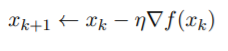
\includegraphics{gradient descent.png}, where $\eta$ is some fixed step size." While the popular science resource glosses over the types of problems that gradient descent encounters difficulty in solving, the paper describes it clearly: if the gradient is zero at some point, there is no escape and gradient descent can at best find a stationary point, which may be a local minimum, but could also be a saddle point or a local maximum. The paper investigates the complexity of finding a point where the gradient descent algorithm terminates when the domain is bounded. When the domain is bounded, a point of this type is guaranteed to exist, and can be verified efficiently and necessarily exists. This places gradient descent squarely into the TFNP class, but the paper goes on to describe the formal definitions of PPAD, PLS, and CLS, all syntactic subclasses of TFNP. By proving that gradient descent is PPAD $\cap$ PLS, the authors demonstrate convincing evidence that gradient descent is a hard problem in itself. Further, the authors state, "PPAD $\cap$ PLS is the class of all problems that can be solved by performing Gradient Descent on a bounded domain," which demonstrates that PPAD $\cap$ PLS is a class of problems that are not simply artificial, but support interesting and important applications.

The popular science news article was found here: 

Thieme, N. (2021, August 29). Computer scientists find a key research algorithm's limits. Wired. Retrieved November 16, 2021, from https://www.wired.com/story/computer-scientists-find-a-key-research-algorithms-limits/. 

The primary source research paper was found here:  

Fearnley, J., Goldberg, P. W., Hollender, A., \&; Savani, R. (2021). The complexity of gradient descent: CLS = PPAD $\cap$ PLS. Proceedings of the 53rd Annual ACM SIGACT Symposium on Theory of Computing. https://doi.org/10.1145/3406325.3451052 

\collab{None}
\nextprob{Decrementing Function}

Prove that the generic algorithm for SSSP, \textsc{FordSSSP}, terminates using a
decrementing function.

\paragraph{Answer}
Let G = (V, E, w) where V is the set of vertices, E is the set of edges, and w are weights on the edges. A tense edge is an edge for which the tentative shortest path is clearly incorrect; if $d[u]+w(u,v) < d[v]$, then $d[v]$ should be replaced. Let $T$ be the set of tense edges (T $\in$ E). The while loop in $FordSSSP$ stating, "while there is at least one tense edge" can be rewritten to iterate over the collection of tense edges. Thus the while loop becomes "for $i$ in the set of tense edges (for $i \in T$). Then we can define a decrementing function $d : \mathcal{S} \rightarrow S$ to be $d(*) = T - i$, where $i$ is some tense edge in the set of tense edges $T$. 

Because $d(*) = T - i$ exists and $\mathbb{N}$ is well-ordered, min(im(d)) is realized, which means that the algorithm terminates.

\collab{None}
\nextprob{All Pairs Shortest Paths}

Walk through \textsc{ShimbelAPSP} algorithm (Erickson, page 314) for the graph given in class on
11/10/21.

\paragraph{Answer}

The ShimbelAPSP algorithm found on page 314 is the following (with beautifully-drawn line numbers): 

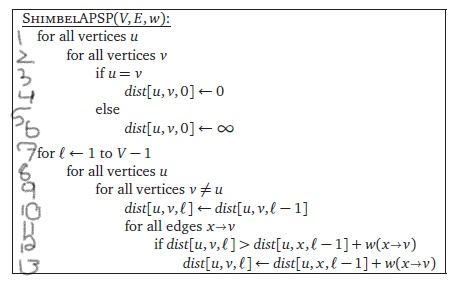
\includegraphics[scale=0.5]{shimbelapsp.jpg}

We will walk through on the following graph with the associated weights per edge.

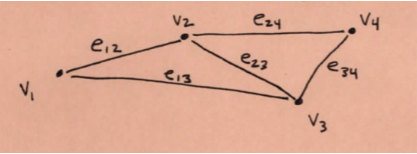
\includegraphics{graph.png}
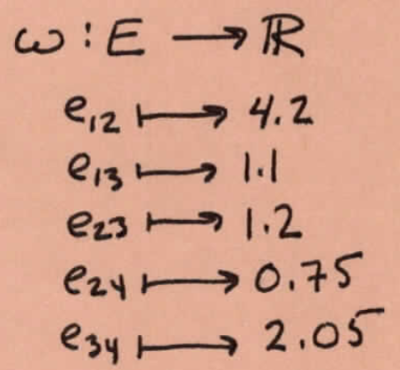
\includegraphics[scale=0.5]{weights.png}

$l$ indicates the number of edges we may traverse to reach another vertex, bounded by one less than the number of vertices ($V - 1$).We begin by initializing the table $l = 0$ in lines 1 through 6. For each vertex that is equal to itself, the $l = 0$ table is assigned 0, and for each vertex different, it is assigned infinity. At this point in the algorithm, we haven't begun to explore whether a path exists between each vertex and another; all we can definitively say is that if you are at the vertex you're attempting to reach, the distance is 0.

\begin{table}[]
\begin{tabular}{|l|l|l|l|l|}
\hline
$l = 0$  & $v_1$                  & $v_2$                  & $v_3$                  & $v_4$                  \\ \hline
$v_1$ & 0                     & $\infty$ & $\infty$ & $\infty$ \\ \hline
$v_2$ & $\infty$ & 0                     & $\infty$ & $\infty$ \\ \hline
$v_3$ & $\infty$ & $\infty$ & 0                     & $\infty$ \\ \hline
$v_4$ & $\infty$ & $\infty$ & $\infty$ & 0                     \\ \hline
\end{tabular}
\end{table}

Now, we consider $l = 1$: what paths exist between each pair of vertices using only one edge? This step corresponds to line 7, where $l = 1$. In line 9 (for all vertices that do not equal itself), we tentatively mark each distance from $u$ to $v$ as equal to the previous distance from the $l - 1 = 0$ table (line 10). In this case, the "tentative" table looks the same as $l = 0$. Then we iterate through all edges connected to the vertex of interest (line 11) and replace the infinities with the shortest distance that is possible using only one edge. Note that because it is impossible to reach vertex 4 from vertex 1, that the infinities stay in that place. 

\begin{table}[]
\begin{tabular}{|l|l|l|l|l|}
\hline
$l = 1$  & $v_1$                  & $v_2$                  & $v_3$                  & $v_4$                  \\ \hline
$v_1$ & 0                     & 4.2 & 1.1 & $\infty$ \\ \hline
$v_2$ & 4.2 & 0                     & 1.2 & 0.75 \\ \hline
$v_3$ & 1.1 & 1.2 & 0                     & 2.05 \\ \hline
$v_4$ & $\infty$ & 0.75 & 2.05 & 0                     \\ \hline
\end{tabular}
\end{table}

We now consider $l = 2$: what path is the shortest between each pair of vertices using up to two edges? This step corresponds to line 7, where $l = 2$. In line 9 (for all vertices that do not equal itself), we tentatively mark each distance from $u$ to $v$ as equal to the previous distance from the $l - 1 = 1$ table (line 10). In this case, the "tentative" table looks the same as $l = 1$. Then we iterate through all edges connected to the vertex of interest (line 11) and replace the infinities with the shortest distance that is possible using up to two edges. In this step, $v_1 \rightarrow v_2$ is replaced with 2.3, the sum of the weights of $e_{13}$ and $e_{23}$, because these weights are smaller than weight 4.2 of edge $e_{12}$. $v_3$ to $v_4$ is replaced by a lesser-weight distance of 1.95, formed by summing the weights of $e_{23}$ and $e_{24}$. Traversing from $v_1$ to $v_4$ is also possible using two edges, $e_{13}$ (w = 1.1) and $e_{34}$ (w = 2.05) for a sum of 3.15, which replaces the infinities. 

\begin{table}[]
\begin{tabular}{|l|l|l|l|l|}
\hline
$l = 2$  & $v_1$                  & $v_2$                  & $v_3$                  & $v_4$                  \\ \hline
$v_1$ & 0                     & 2.3 & 1.1 & 3.15 \\ \hline
$v_2$ & 2.3 & 0                     & 1.2 & 0.75 \\ \hline
$v_3$ & 1.1 & 1.2 & 0                     & 1.95 \\ \hline
$v_4$ & 3.15 & 0.75 & 1.95 & 0                     \\ \hline
\end{tabular}
\end{table}

We now consider $l = 3$: what path is the shortest between each pair of vertices using up to three edges? This step corresponds to line 7, where $l = 3$. In line 9 (for all vertices that do not equal itself), we tentatively mark each distance from $u$ to $v$ as equal to the previous distance from the $l - 1 = 2$ table (line 10). In this case, the "tentative" table looks the same as $l = 2$. Then we iterate through all edges connected to the vertex of interest (line 11) and replace the infinities with the shortest distance that is possible using up to two edges. The only improvement over $l = 2$ by the use of 3 edges is the shortest path from $v_1$ to $v_4$, 

\begin{table}[]
\begin{tabular}{|l|l|l|l|l|}
\hline
$l = 3$  & $v_1$                  & $v_2$                  & $v_3$                  & $v_4$                  \\ \hline
$v_1$ & 0                     & 2.3 & 1.1 & 3.05 \\ \hline
$v_2$ & 2.3 & 0                     & 1.2 & 0.75 \\ \hline
$v_3$ & 1.1 & 1.2 & 0                     & 1.95 \\ \hline
$v_4$ & 3.05 & 0.75 & 1.95 & 0                     \\ \hline
\end{tabular}
\end{table}

\end{document}
